\documentclass[14pt]{extarticle}
\usepackage[T1]{fontenc}
\usepackage[utf8]{inputenc}
\usepackage[colorlinks=true,urlcolor=blue,linkcolor=black]{hyperref}
\usepackage[scaled]{uarial}
\usepackage[colorlinks=true,urlcolor=blue,linkcolor=black]{hyperref}
\usepackage[scaled]{uarial}
\usepackage{graphicx}
\usepackage{float}
\renewcommand*\familydefault{\sfdefault} %% Only if the base font of the document is to be sans serif
\date{}
\begin{document}
\title{Microservices - Group 3}
\author{Pedro Carrega, nº49480 \and
Vasco Ferreira, nº49470 \and Ye Yang, nº 49521
}
\maketitle
\tableofcontents
\newpage
\section{From Monolith to Microservices: A Classification of Refactoring Approaches}
\subsection{Introduction}
This paper focuses on comparing refactoring approaches of pre-existent monolithic architecture services to a microservices based architecture in order to make the most out of the scalability and efficiency this type of architecture offers.

As seen throughout the course, microservices bring many advantages over traditional monolithic architectures through non functional characteristics such as elasticity, scalability, redundancy, among others.
Monolithic applications become larger and more complex overtime, having the entirety of its source code distributed on a single system. This makes it hard for developers to debug their code and thus making it hard to maintain.

However, the re implementation of the system with a microservices architectures is no easy feat, as one has to take into account how to partition the source code not only logically, but also regarding exterior factors in the real world as we will further address. The correct deployment of a system with such an architecture will depend on the correct refractoring and decomposition of the system.

\subsection{Refractoring}
When refractoring an application, we must not only consider code level refractoring, but also architectural refractoring. This is mainly due to most organizations building a system according to its own communication structure, thus both the system's architecture and the organization are interdependent making the refractoring process not only code based.

We must however, also take into account the granularity of the services in which the monolithic application will be decomposed into, so as not to overload some services and underload others due to improper task distribution. Two ways to split the system into smaller parts are underlined in the paper:
\begin{itemize}
	\item \textbf{Implementation Technology} - separation of the monolithic system into smaller subsystems based on the level of computation (ex.: Heavy services written in C into one subsystem and IO-heavy services written in NodeJS in another subsystem).
	\item \textbf{Geography} - separating the system based on the physical location of each development team, whether it be due to commercial, cultural, legal or technical reasons.
\end{itemize}

To gather the data regarding the refractoring techniques in microservices, the authors queried papers with specific keywords on three of the largest libraries of scientific papers in computer science: IEEE, ACM Digital Library and Google Scholar.

\subsection{Results}
With the data obtained from the three libraries, only 10 were selected, as most others focused on the requirements of a specific scenario, without much theoretical basis, not being able to generalize their approaches for other systems.

The various approaches from the 10 selected can be categorized in 4 main decomposition strategies which take into account external factors, not only based on source code, as input in order to determine the granularity of each service offered. The strategies are the following:
\begin{itemize}
	\item \textbf{Static Code Analysis aided} - primarily based on studying the source code of the application and logically decomposing it into smaller subsystems.
	\item \textbf{Meta-Data aided} - based on the architecture of the system, aided by UML diagrams and use cases. More abstract than Static Code Analysis.
	\item \textbf{Workload-Data aided} - based on the computational power required for the application in order to determine its decomposition (ex.: communication, performance).
	\item \textbf{Dynamic Microservice Composition} - in which we define a microservice runtime environment best suited for each set of services. This environment is subject to change with each composition re-calculation iteration in order to find the best fit for each service.
\end{itemize}

In Figure 1 we can see a decision graph made by the authors so as to simplify the choosing of the best option for specific type of application to be refractored. The decomposition approaches are best viewed directly from the paper which can be accessed through the following link: \url{https://arxiv.org/ftp/arxiv/papers/1807/1807.10059.pdf}

\begin{figure}[H]
  \centering
    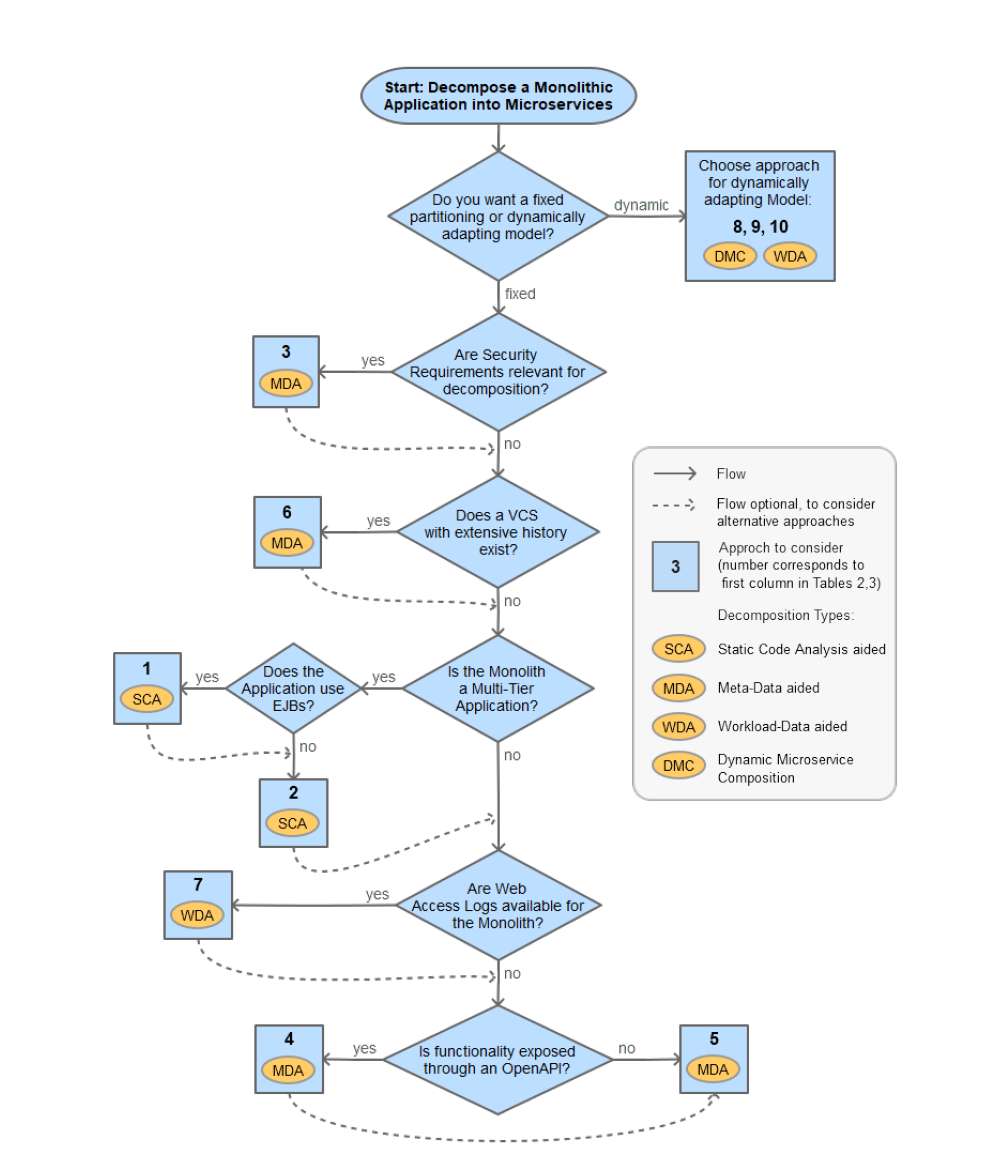
\includegraphics[scale=0.5]{Decision_Graph.png}
  \caption{Decision Guide}
\end{figure}
\noindent

\subsection{Conclusion}
In the presented paper, the amount of proposed strategies for application refractoring and decomposition are limited and although more generic than the papers that were filtered out, limitations to universal adaptability are still present. Nevertheless it is a solid baseline which can be used to refractor basic level applications, small to medium sized. Enterprise sized applications would have to apply a more sophisticated method that best caters to their specific scenario.

\section{Research on optimization of course selection system based on micro service and dynamic resource extension}
\subsection{Introduction}
In the academic world the course selection systems have been using remote technologies for some time, that way it is possible for students to enroll in the courses when they want and where they want. This is a better approach to the institution since course selection would require a huge amount of staff and would take more time for all students to enroll. 
Has expected, all this remote course selection has its problems, in most of the educational institutions where it is implemented, there is the problem of servers crashing during the process due to the huge amount of students concurrently accessing the services. 
The institution could use vertical scalability, by upgrading their servers so that it could support a bigger amount of concurrent requests. But this approach as it will be shown could be unfeasible since it will have an associated monetary cost.

To tackle this reoccurring problem three students from the Guangzhou University though to optimize the architecture of the system instead of maintaining the same but improving the servers. Their idea was to deploy a micro-services architecture, separating all the business logic by micro-services, where there are the following benefits:
\begin{itemize}
 	\item Easier to develop and maintain
	\item Local modifications are easier to deploy
	\item Easier to scale the necessary services
\end{itemize}

To follow this approach, it was needed to re-design the system architecture.
\subsection{System Architecture}
\begin{figure}[H]
  \centering
    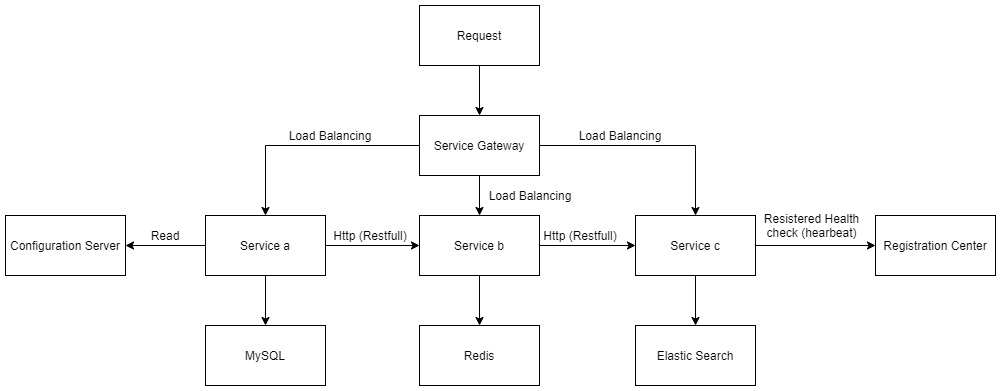
\includegraphics[scale=0.4]{ArqFig1.jpg}
  \caption{System Architecture}
\end{figure}
\noindent
\textbf{Registration Center:} This component is used to standardize the information of the various micro-services, provide query API for querying available instances and the manage API for service registration, cancellation, discovery and service inspection (heartbeat mechanism).

\noindent
\textbf{Service Gateway:} It is used provide a better access point to the client, abstracting all the underlying structure of the application.

\noindent
\textbf{Configuration Server:} Since some services are dependent on another the configuration server is needed for a centralized management configuration.

\noindent
\textbf{Redis Cluster:} Some necessary information is pre-stored in Redis. After the class selection the data in memory is store in the database by timing tasks, to achieve Redis pressure resistant property.

\noindent
\textbf{Distributed Tracking:} By combining the elastic search with course log analysis system and micro-services can solve problems in time to avoid larger problems.

\subsection{Micro Services}
A service implementation mainly includes business logic, data storage, adapter, and service interface. The database adapter is useful to adapt different services to different databases, so that it facilitates the migration of services in different database environments. Database servers provide data storage support for micro-services to ensure the atomicity and independence of services.
\begin{figure}[H]
  \centering
    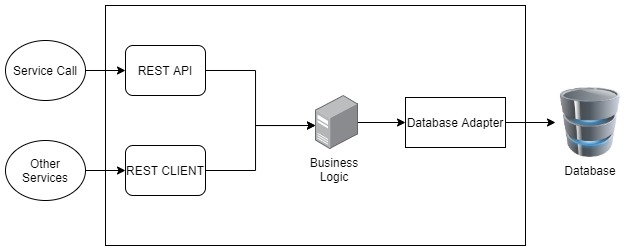
\includegraphics[scale=0.65]{Micro-service.jpg}
  \caption{Micro Service Implementation}
\end{figure}

\subsection{Results and Conclusion}

After all the implementation the students accomplished a huge improvement in each service, due to the benefits of micro-services that were mentioned before. With the monolith, the institution servers would struggle with only 3000 to 4000 concurrent users. After the implementation the students were faced with the following results:
\begin{table}[H]
	\begin{center}
		\begin{tabular}{|p{4.8cm}|p{3.8cm}|p{5.4cm}|}
		\hline
			\textbf{Number of\newline concurrent users} & \textbf{Transaction\newline success rate} & \textbf{Average transaction\newline response time}\\ \hline
			4000 & 100\% & 1.314 seconds\\ \hline
			10000 & 100\% & 2.52 seconds\\ \hline
			15000 & 100\% & 7.011 seconds\\ \hline
	\end{tabular}
	\label{tab2}
	\end{center}
	\caption{Results with micro-services}
\end{table}

With the following results we can determinate that the application was a success, that the problem was not the hardware it self, but the architecture that defined the system. By changing it to micro-services all the transactions were successful which is the main goal, but also the average transaction times were very low which provides a better user experience.

The goal is not to say that micro-services is always the way to go, but when applied in the correct scenario, applications can benefit enormously due to its properties, like on demand scalability of services, adjusting the number of nodes running certain services that are experiencing a high load while some services are not having any load at all.

To understand more of the evaluation done in the course selection system, visit the following link to read the paper: \url{https://dl.acm.org/doi/abs/10.1145/3335484.3335546}

\section{Microservice Architectures for Scalability, Agility and Reliability in E-Commerce}

\subsection{Introduction}

The focus of this paper is to present different properties of microservice architectures using the platform \textit{otto.de} as example. Traditional systems usually operate on a monolithic architecture, using an integrated databases, however this greatly limits the horizontal scalability of said databases. A microservice architecture tries to overcome that limitation, providing an architecture composed of multiple smaller microservices where typically there is no central control. Microservices are built around business capabilities and take a full-stack implementation of software. To comprehend the rest of the paper the following topics must be understood.

\subsubsection{Vertical Decomposition for Microservices}

When using many small microservices the correct level of granularity must be taken into account. The author proposes using an vertical decomposition into self contained systems along business services. This provides the system with scalability, an appropriate modular structure that supports program comprehension, resilience and autonomous teams with good knowledge of their vertical domain.

\subsubsection{Loose Coupling and Eventual Consistency}

Where monolithic systems use transactions when updating their systems, do to the low coupling usually found on microservices, implementing the same update system is very difficult. And as such, microservice architectures emphasize transaction-less between services and that most problems must be resolved with compensation operations.

\subsubsection{Microservices for Scalability and Fault Tolerance}

Microservices must be designed so that they can tolerate the failure of individual systems. It's important to be able to detect failures quickly, and if possible, restore services automatically. Emphasizing real-time monitoring, using both technical metrics and business metrics, we are able to receive early warnings of possible problems along a faster follow up time by the development team. Microservices can be dynamically replicated when the system is under heavy load, providing an high level of elasticity and scalability.

\subsubsection{Microservices and DevOps}

With the goal of improving communication between developers (Dev) and IT operations (OPS), the DevOps movement uses automation to build systems, execute unit tests and deployment in test and production environments.

\subsubsection{Scalable Microservice Deployment}

Containerization complements very well microservices, due to it's low overhead when compared with virtualization. A cluster infrastructure schedule containers onto nodes in a cluster and manage load balancing among containers.

\subsubsection{Scalable Microservices Deployment}

Microservices reinforce a modular structure, making the decoupling of teams as important as the decoupling of software modules.

\subsection{Microservices at \textit{otto.de}}

Otto started a complete re-implementation of their e-commerce software in 2011. This decision was driven by the need of a more scalable and fault tolerant system. This would not only apply to the system in question but to the teams surrounding it as well, with the practice of DevOps in the forefront.
The development of a vertically decomposed system was initiated by four teams, with each team assign to one of the four initial applications:
\begin{itemize}
	\item Product
	\item Order
	\item Promotion
	\item Search/Navigation
\end{itemize}

In the following image we are able to see the current "verticals" at Otto, with 18 teams working on 45 applications.

\begin{figure}[H]
	\centering
	  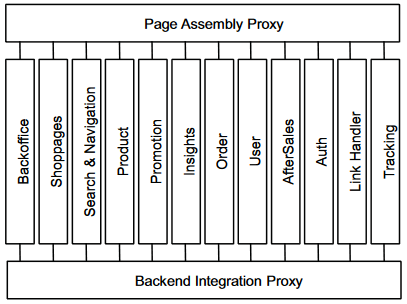
\includegraphics[scale=0.5]{vertical_decomposition.png}
	\caption{Vertical Decomposition at \textit{otto.de}}
  \end{figure}

A vertical represents a single context in the business domain within the platform. While they can be as small as a microservice, usually they are more coarse grained. Communication between verticals is only allowed by using the REST API, protecting working applications from a possible snowball effect from unavailable applications.

Nothing is shared between verticals, each using each own databases and resources. Using cookies to share the client-side state between different systems. This grants the system excellent horizontal scalability and fault tolerance.

%preciso de por 1 frase a introduzir esta parte

\begin{itemize}
	\item \subsubsection{Intergating Verticals at \textit{otto.de}} 
	Each vertical contains fragments from other verticals so that the client experiences a full product despite the decomposition at the backend.
	\item \subsubsection{Communication among Verticals at \textit{otto.de}}
	All verticals have redundant data using pull-based data replication, allowing a vertical to deliver content without having to request other verticals.
	\item \subsubsection{Scaling Delivery Pipelines at \textit{otto.de}} 
	The system is updated very frequently using pipelines. All commits follow the same cycle: first it's checked out, then compiled and packaged, then deployed and tested. Using run load and integration tests so that the product owners approve the stories. The last step the service is tested against other live services to check compatibility.
	\item \subsubsection{Agility and Reliability at \textit{otto.de}} 
	Using the DevOps movement, every push is automatically deployed. This deployment system lead to a reduction of incidents throughout the years, even with the significant increase of deployments.
	\item \subsubsection{Monitoring Microservices at \textit{otto.de}}
	Every team receives real time graphs and metrics for all microservices and verticals. With the increasing number of active microservices, it is planned to develop solutions so that anomalies can be automatically detected.
	\item \subsubsection{Dynamic Scaling of Microservices at \textit{otto.de}}
	By monitoring CPU utilization and the number of incoming requests, the system is capable of automatically replicate it's features.
	\item \subsubsection{Code Sharing and Reuse at \textit{otto.de}}
	No code is shared among microservices in order to have low coupling between microservices, only the framework of the code can be reused. The only exceptions to this rule is code determined to be loosely coupled and highly coherent. This code is made open source and all teams are free to use it.
\end{itemize}

\subsection{Conclusion}

Microservices architectures creates scalable, agile and reliable software systems. Using a vertical decomposition it provides the basis of highly scalable and reliable system. By following this ideals the team at \textit{otto.de} managed not only to create a scalable system but also a scalable deployment. That doesn't mean the microservices are perfect. It comes with a high learning and maintenance cost due to it's constant need of consistency, monitoring, alarming and fault tolerance. Making it, albeit an ideal system for most scenarios, a complex system to implement and maintain.

\end{document}
